\chapter{Vehicle Detection Module}  \label{kap:vehicle-detection}

Object detection is an important problem appearing on many science fields and
applications like for example robotics, medical science, surveillance systems, etc. The
goal is to detect or determine the presence of a particular object of interest
given a set of measurements obtained from sensors. In the particular context of
computer vision, cameras are commonly used as the sensors and the images they
produce are the measurements.

In this project one of our interest is precisely to detect objects in images 
obtained form a cellphone camera. Specifically we want to detect vehicles and 
be able to get the distance between them and the camera. In this
chapter we are going to present the theory and the method that was considered to
tackle this problem.

\section{Object detection and image classification} % (fold)
\label{sec:objectdetec}

In this section we are going to get through the theoretical framework involved
in the process of detecting objects in camera images. As the reader may know,
there does not exist a definite solution to this problem due to its inherent
complexity. Through the years many interesting strategies have being proposed to
tackle this problem and some of them have shown very good results.

In particular, the work of \cite{viola-jones} in face detection is very
important inside the computer vision community and is the origin for many state
of the art methods used nowadays for object detection. The idea of this work was
to use Machine Learning techniques to learn the intrinsic properties of the
underlying texture produced by a particular object in a image. These underlying
properties are extracted using \textit{features} which consequently are
used to \textit{classify} a texture.

For this project, our goal is to find the set of features that describe the
texture produced by a vehicle and classify those regions in the image with these
features as the detected vehicles. We start by defining the type of features
that are going to be extracted from the images, then we will describe the
machine learning algorithm used to extract the particular subset of feature that
describe a vehicle and finally some words about the data used in the learning
process.

\subsection{Feature calculation} % (fold)
\label{sub:Features}

In computer vision and image processing, the term \textit{feature} is commonly 
used for structures or pieces of information that are relevant when analysing an
image. There are uncountable examples of features that can be extracted from an 
image like points, edges, areas, averages of intensities, etc. A particular set
of features and the way to extract them from the image may vary depending on the
application.

For object detection, the set of features used should be robust to capture and
describe the particular textural properties produced by the object of interest.
A particular example in the work of \cite{viola-jones} for face detection, they 
use the well known \textit{Haar-like} features. These features basically compare
the intensity of different regions in the image. This is a particular good
choice of features because when thinking about faces in general, regions like 
the forehead and nose tend to be more illuminated than the region of the eyes 
or beneath the nose. 

Altough Haar-like features have been used in vehicle detection applications, we
opt by using other type of features called \textit{Local Binary Patterns}. First
propposed by \cite{ojala}, the LBP features are one of the best texture
descriptors. They have proven to be highly discriminative and their key advantages,
namely, their invariance to monotonic gray-level changes and computational
efficiency, make them perfect for real-time image processing applications.

The basic idea of LBP features is to summarize the local structure in an image
by comparing each pixel with its neighborhood. For instance, each pixel in the 
neighborhood is compared in terms of intensity to the central pixel. If the
intensity value is higher than the central pixel, it is marked as 1 and 0
otherwise. At the end of the process the neighborhood of each pixel will have a
binary pattern. This basic process is ilustrated in the figure~\ref{fig:lbp}. 

\begin{figure}
\begin{center}
    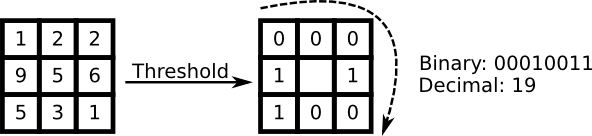
\includegraphics[scale=1.0]{img/lbp.png}
\end{center}
\caption{Ilustrated example in the calculation of the Local Binary Pattern for a
pixel with neighborbood of size 8.}
\label{fig:lbp}
\end{figure}

More formally the LBP extraction can be defined as an operator in the following
manner

\begin{equation*}
    LPB(x_c, y_c) = \sum^{P-1}_{p=0}{2^ps(i_p - i_c)}
\end{equation*}

Where $(x_c, y_c)$ are the coordinates if the central pixel. The intensity of
the central pixel $i_c$ is thresholded with the intensity $i_p$ of the neighbor
$p$ through the function $s$ defined as 

\begin{equation*}
    s(x) =
    \begin{cases}
        1        & \text{if } x \geq 0 \\
        0        & \text{otherwise}
    \end{cases}
\end{equation*}

Finally the binary pattern is stored in form of decimal suming the corresponding
powers of 2.

Nevertheless this simple operator is to illustrate the main idea
of LBP because its fixed neighborhood fails to capture details at different
scales. For this reason, there have been many attemps to extend the LBP operator
to overcome this problem. One particular example is in the work of
\cite{ahonen} called \textit{Extended LBP} or \textit{Circular LBP}. This
extension for the LBP considers a arbitrary number of neighbors at a radial
distance from the central pixel. Formally the coordinates for the neighbor pixel
$p$ are expressed as

\begin{align*}
    x_c &= x_c + R \cos(\frac{2\pi p}{p}) \\
    y_c &= y_c - R \sin(\frac{2\pi p}{p}) \\
\end{align*}

Where $R$ is the distance to the central pixel. When these coordinates do not
correspond to image coordinates, the intensity is calculated by a bilinear
interpolation. In the figure~\ref{fig:lbp-invariant} is reflected the property
of this operator of being invariant to monotonic changes in the intensity.

To incorporate the spatial information, \cite{ahonen} proposed to divide the
image in uniform regions and extract from each one a histogram of the binary
patterns. The histograms from each region are concatenated to form the final
feature vector of the image. This feature vector is also known as
\textit{Local Binary Patterns Histograms}.

\begin{figure}
\begin{center}
    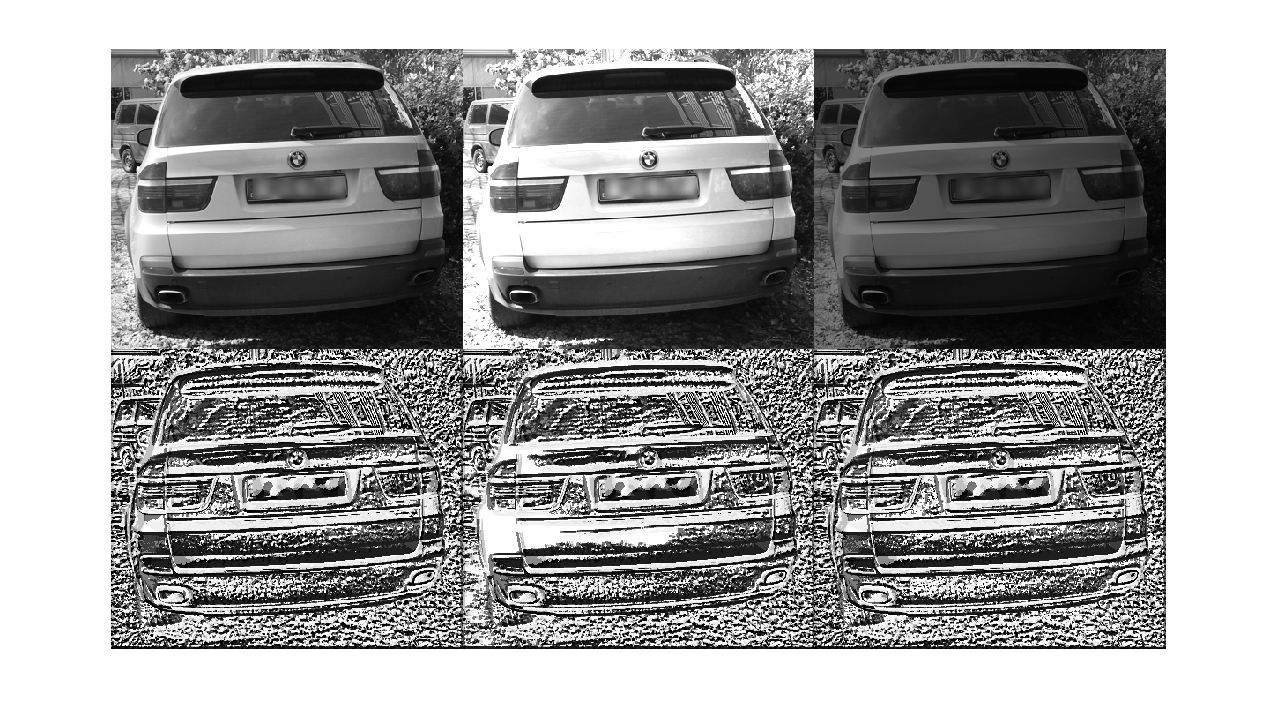
\includegraphics[scale=0.3]{img/invariance.png}
\end{center}
\caption{Local Binary Patterns invariance to constant intensity changes}
\label{fig:lbp-invariant}
\end{figure}

% subsection Features (end)


\subsection{Feature learning} % (fold)
\label{sub:feature-learning}

In the previous section we explained the type of features that are extracted
from the images. The next step is to learn which group of them better describe
the object we are interested in. In order to do this, we used a Machine Learning
algorithm. In particular, in the work of \cite{viola-jones} they used the
\textit{Adaboost} algorithm. 

Short for ``Adaptive Boosting'', this algorithm was first proposed by
\cite{freund}. In this particular type of boosting, \textit{weak} classifiers
are collected iteratively in a way they adapt to the errors of previously
selected classifiers. The final \textit{strong} classifier is build based on the
votes of each weak classifiers. 

Weak classifier is a name commonly used in Machine Learning to denote hypothesis 
functions that perform slightly better than random in the \textit{training data
set}. In other words, given a set of mixed pictures of vehicles and non-vehicles, a
weak classifier should be able to separate them in a way that the number of
correctly classified pictures is slightly larger than the incorrect ones. The
classification is perform not directly on the images but in the feature vector
extracted from them.

In the training phase every training example, meaning every picture of a
vehicle or non-vehicle, has a weight associated to it. On each iteration, the
weights of the training examples wrongly classified will increase and the
weights of the correctly classified will decrease. This makes that in each
iteration the selected classifier will be prioritize the correct classification
of those training examples with higher weights. In the figure~\ref{fig:adaboost}
you can find an illustration of this idea.

\begin{figure}
\begin{center}
    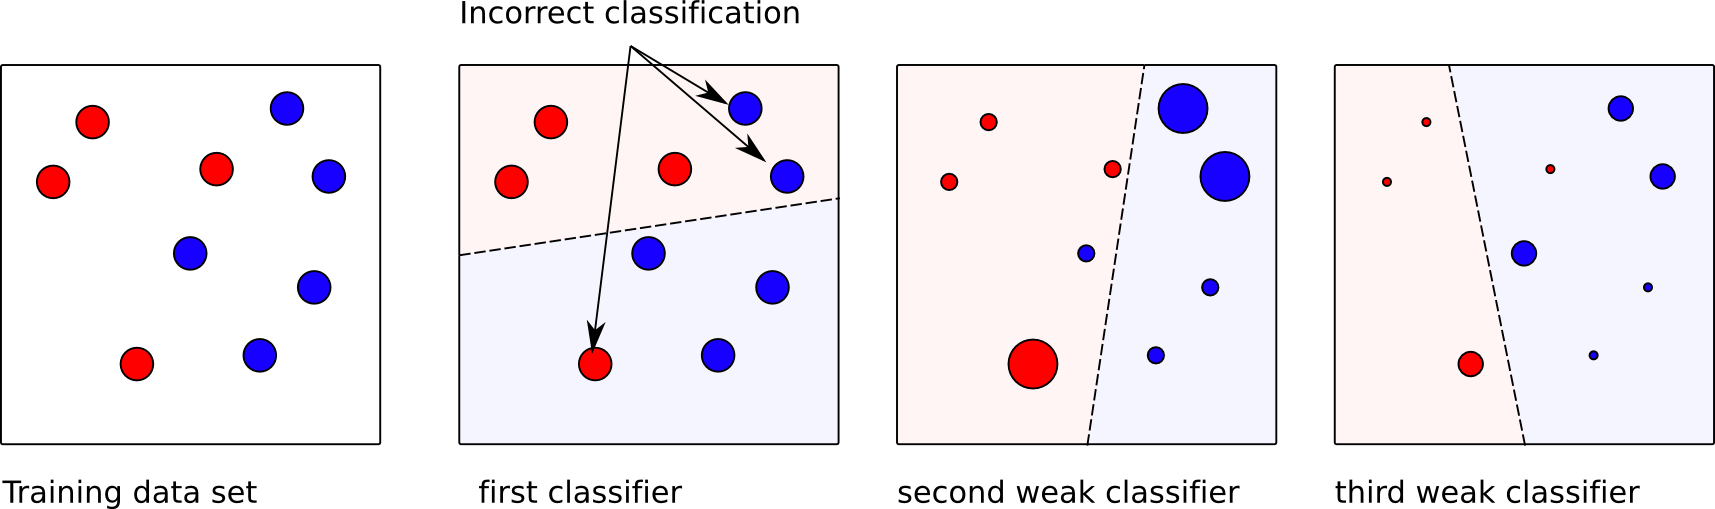
\includegraphics[scale=0.6]{img/adaboost.png}
\end{center}
\caption{Illustration of the AdaBoost algorithm learning. The weak classifiers
are represented by lines separating the training examples in a hypothetical 2D
feature space. The color represents the class of the object and the size of the
points represents the importance weight.}
\label{fig:adaboost}
\end{figure}

Formally the algorithm is described in the table~\ref{alg:Adaboost}. Note how
the final strong classifier is just a weighted sum of the votes of each weak
classifier. The weighting is given by their performance on the dataset.


\begin{algorithm}
    \caption{Adaboost algorithm}
    \begin{algorithmic}[1]
        % \Require Metric space $(X, d_x)$, some initial point $x_1 \in X$ and the
        % desire sampling radius $r_0$.
        % \Ensure a sampling $X' = \{x_1, \dots, x_N\}$.
        \State Initialize the data weighting coefficients $\{w_n\}$ by setting
        $w_n^{(1)} = \frac{1}{N}$ for $n = 1, \cdots, N$.
        \For {$m = 1, \cdots, N$}
        \State \parbox[t]{\dimexpr\linewidth-\algorithmicindent}
        {Fit a classifier $y_m(x)$ to the remaining data by minimizing
        \begin{equation*}
            J_m = \sum^{N}_{n=1}{w_n^{(m)} I(y_m(x_n) \ne t_n)}
        \end{equation*}
        where $I(y_m(x_n) \ne t_n)$ is the indicator function and equals 1
        when $y_m(x_n) \ne t_n$ and 0 otherwise.}

        \vspace{0.25cm}

        \State \parbox[t]{\dimexpr\linewidth-\algorithmicindent}
        {Evaluate the quantities
        \begin{equation*}
            \epsilon = \frac{\displaystyle\sum^{N}_{n=1}{w_n^{(m)}I(y_m(x_n) \ne
        t_n)}}{\displaystyle\sum^{N}_{n=1}{w_n^{(m)}}}
        \end{equation*}
        and then use these to evaluate
        \begin{equation*}
            \alpha_m = \log\left\{ \frac{1 - \epsilon_m}{\epsilon_m} \right\}
        \end{equation*}
        \strut }

        \State Update the data weighting coefficients
        \begin{equation*}
            w_n^{(m+1)} = w_n^{(m)} \exp\left\{ \alpha_mI(y_m(x_n)) \ne t_n \right\}
        \end{equation*}
        \EndFor
        \State \textbf{end}
        \State Make predictions using the final model, which is given by
        \begin{equation*}
            Y_M(x) = sign\left( \sum^{M}_{m=1}{\alpha_m y_m (x)} \right)
        \end{equation*}
    \end{algorithmic}
    \label{alg:Adaboost}
\end{algorithm}


% subsection feature-learning (end)

\subsection{Dataset construction} % (fold)
\label{sub:data-set}

The final step and maybe the most critical one is the dataset construction. In
Supervise Machine Learning everything is about data. The more data we handle,
the more we can learn and the more we can generalize to all possible scenarios.
Unfortunately, gathering data is usually very expensive process. It is expensive
in terms of quality and quantity.

Moreover, depending on the complexity of the application a minimum amount of data 
is required in oder to obtain meaningful results. The higher the complexity of the 
application, the more data is required. In the problem of vehicle detection, we
deal with a high complexity. First of all because the huge variability on
vehicle's shape and color and secondly because of all the factors that can
influence the image formation, like for example weather conditions.

For this work we labeled a set of about 430 pictures of rear view cars. The
pictures where extracted from the dataset used by \cite{tme} and the Caltech
Computer Vision Dataset of rear cars created by Markus Weber (1999). For the
negative examples, we used the Caltech background dataset, also collected by
Markus Weber. Some of the images used as the training dataset are shown in 
the figure~\ref{fig:dataset}.


\begin{figure}[t]
\begin{subfigure}[b]{0.5\textwidth}
\centering
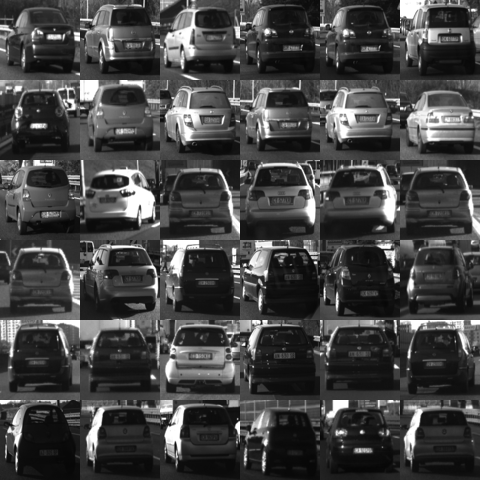
\includegraphics[width=0.85\linewidth]{img/positives.png}
\caption{Positive training examples}
\end{subfigure}
\begin{subfigure}[b]{0.5\textwidth}
\centering
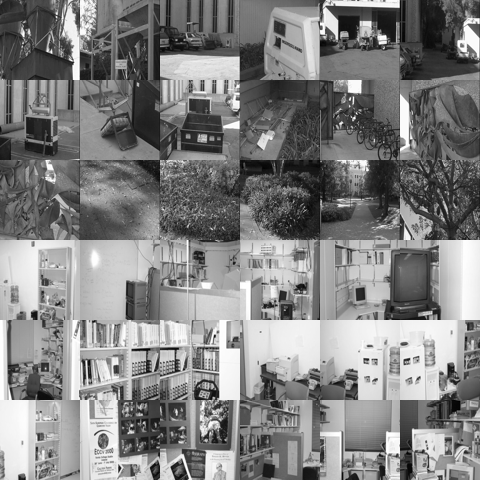
\includegraphics[width=0.85\linewidth]{img/negatives.png}
\caption{Negative training examples}
\end{subfigure}
\caption{Sample of images used as the training set}
\label{fig:dataset}
\end{figure}

% subsection data-set (end)


% section Object detection and image classification (end)

\section{Classification refinement} % (fold)
\label{sec:Classification-refinement}

Due to the great spectrum of different textures appearing in an image, false
classification may occur. This is essentially an inherent problem of the
effort the classifier does to predict unknown data. These mistakes from the
classifier are divided into two types, false positives and false negatives. A
false positives occur when the classifier wrongly label negative examples as 
positive and false negatives is the other way around.

Sometimes it is possible to use some strategies to improve a classification by
removing some of this false classifications. In this particular project, we have
the advantage to work with a continuous flow of images coming from a camera.
This fact offers an extra dimension which allow us to make assumptions in
order to filter some of the false classifications.

Basically we assume the camera is fixed inside the vehicle, meaning that the images
coming from it should show always the frontal view. This summed to the stream of
images allow us to suppose that a vehicle appearing in one image is going to also 
appear in the next one, in almost the same region inside the image.

With this in mind, it is easy to design a simple strategy to eliminate some
false positives. Supposing a vehicle can not simply disappear from one
frame to the other, we can construct a classification window over time, where we
keep track of the position of all the previous classified vehicles. If a new
classification is not consistent with the previous ones in the window, then it
is simply dropped. 

The final size of the region containing the vehicle is averaged with the
information inside the classification window. This smooths jumps of the region
size returned by the classifier due to the search in different scales.

\begin{figure}    
\begin{minipage}[t]{0.45\textwidth}
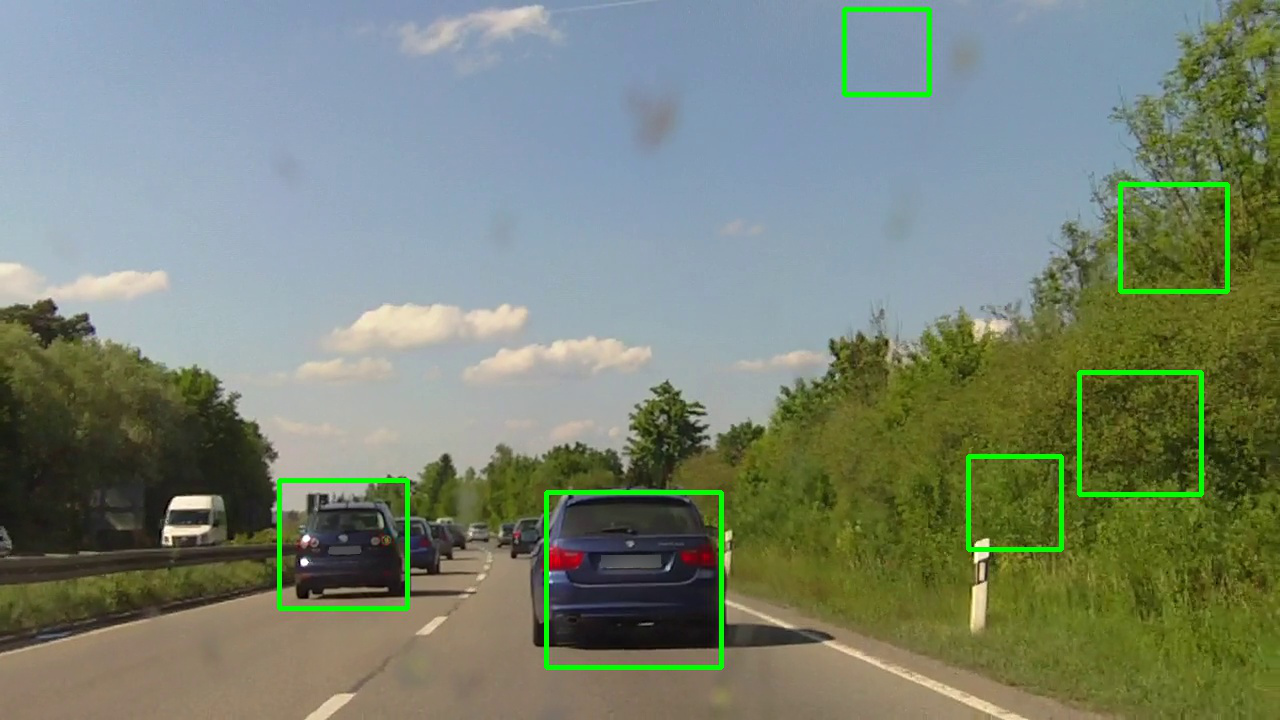
\includegraphics[width=\linewidth]{img/outliers_original.jpg}
\caption{Original classification of the image.}
\end{minipage}
\begin{minipage}[t]{0.45\textwidth}
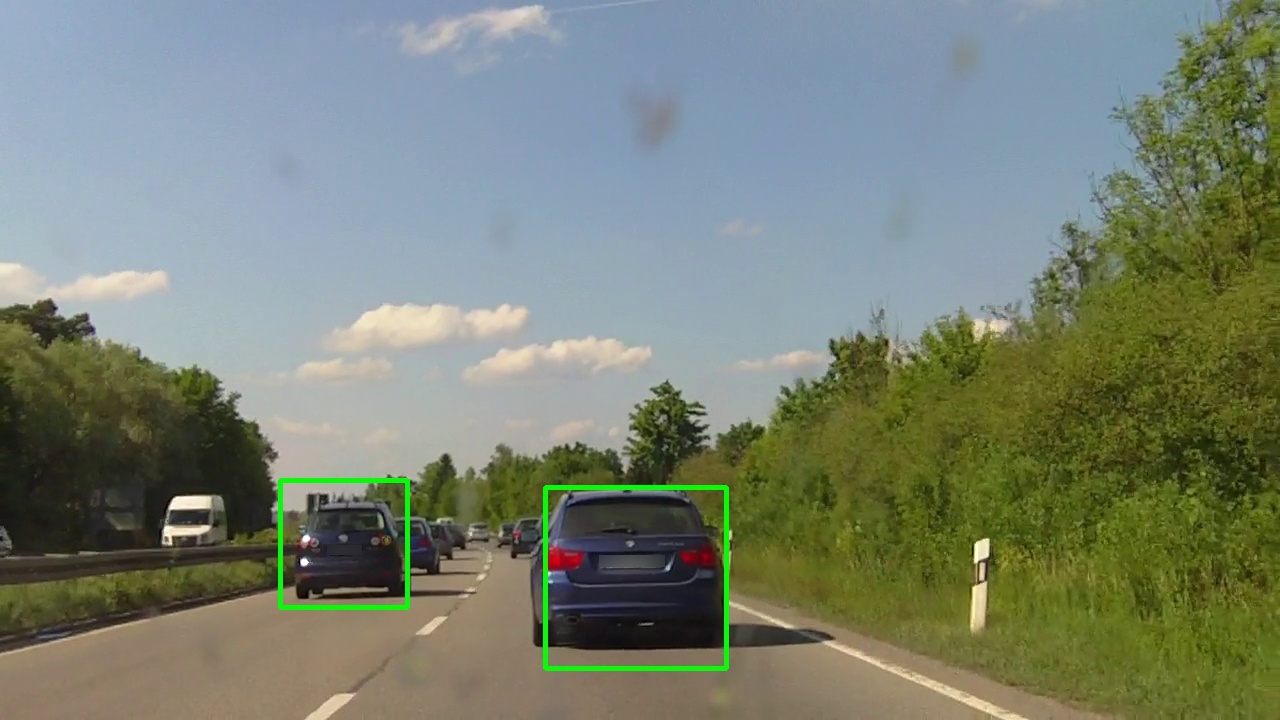
\includegraphics[width=\linewidth]{img/outliers_filtered.jpg}
\caption{False positives filtered with time window strategy}
\end{minipage}
\caption{False positives filtering}
\label{fig:distance-pictures}
\end{figure}

% section Classification refinement (end)

\section{Distance estimation} % (fold)
\label{sec:Distance-estimation}

When projecting the real 3D world through the lenses of a camera into a 2D
image, some information is lost. In particular, the scale and the notion of
distances is lost. It is not possible give any real
measurement of distances in the real world just looking at one image. 
Of course, as humans we can find references in an image from objects we already
know and stablish some scale to compare the rest of the image content. Think for
example of a picture of a small toy car. If the model is realistic 
enough, a human can not differentiate it from a real one, then having an
incorrect estimate of its size.

We face this problem in this section and it is required to make some
assumptions to be able to approximate a solution. First it is assumed that the
pictures we are going to be working with are from real vehicles, this is really
important because our goal is to obtain references of real world distances. The
problem is that generally vehicles have different sizes and shapes. Nevertheless
is not a bad idea to assume an average width for all the vehicles. 

The second problem is that the width in meters of the vehicles is not obtained 
directly from the picture, but a group of pixels containing the image of
the car. To solve this, is necessary to find the relation between the size of
the region containing the vehicle, and the distance to it. For this reason, as a first
approach, we took a number of pictures at different distances of a vehicle. Some of 
these pictures appear in the figure~\ref{fig:distance-pictures}.

\begin{figure}[t]
\begin{subfigure}[b]{0.5\textwidth}
\centering
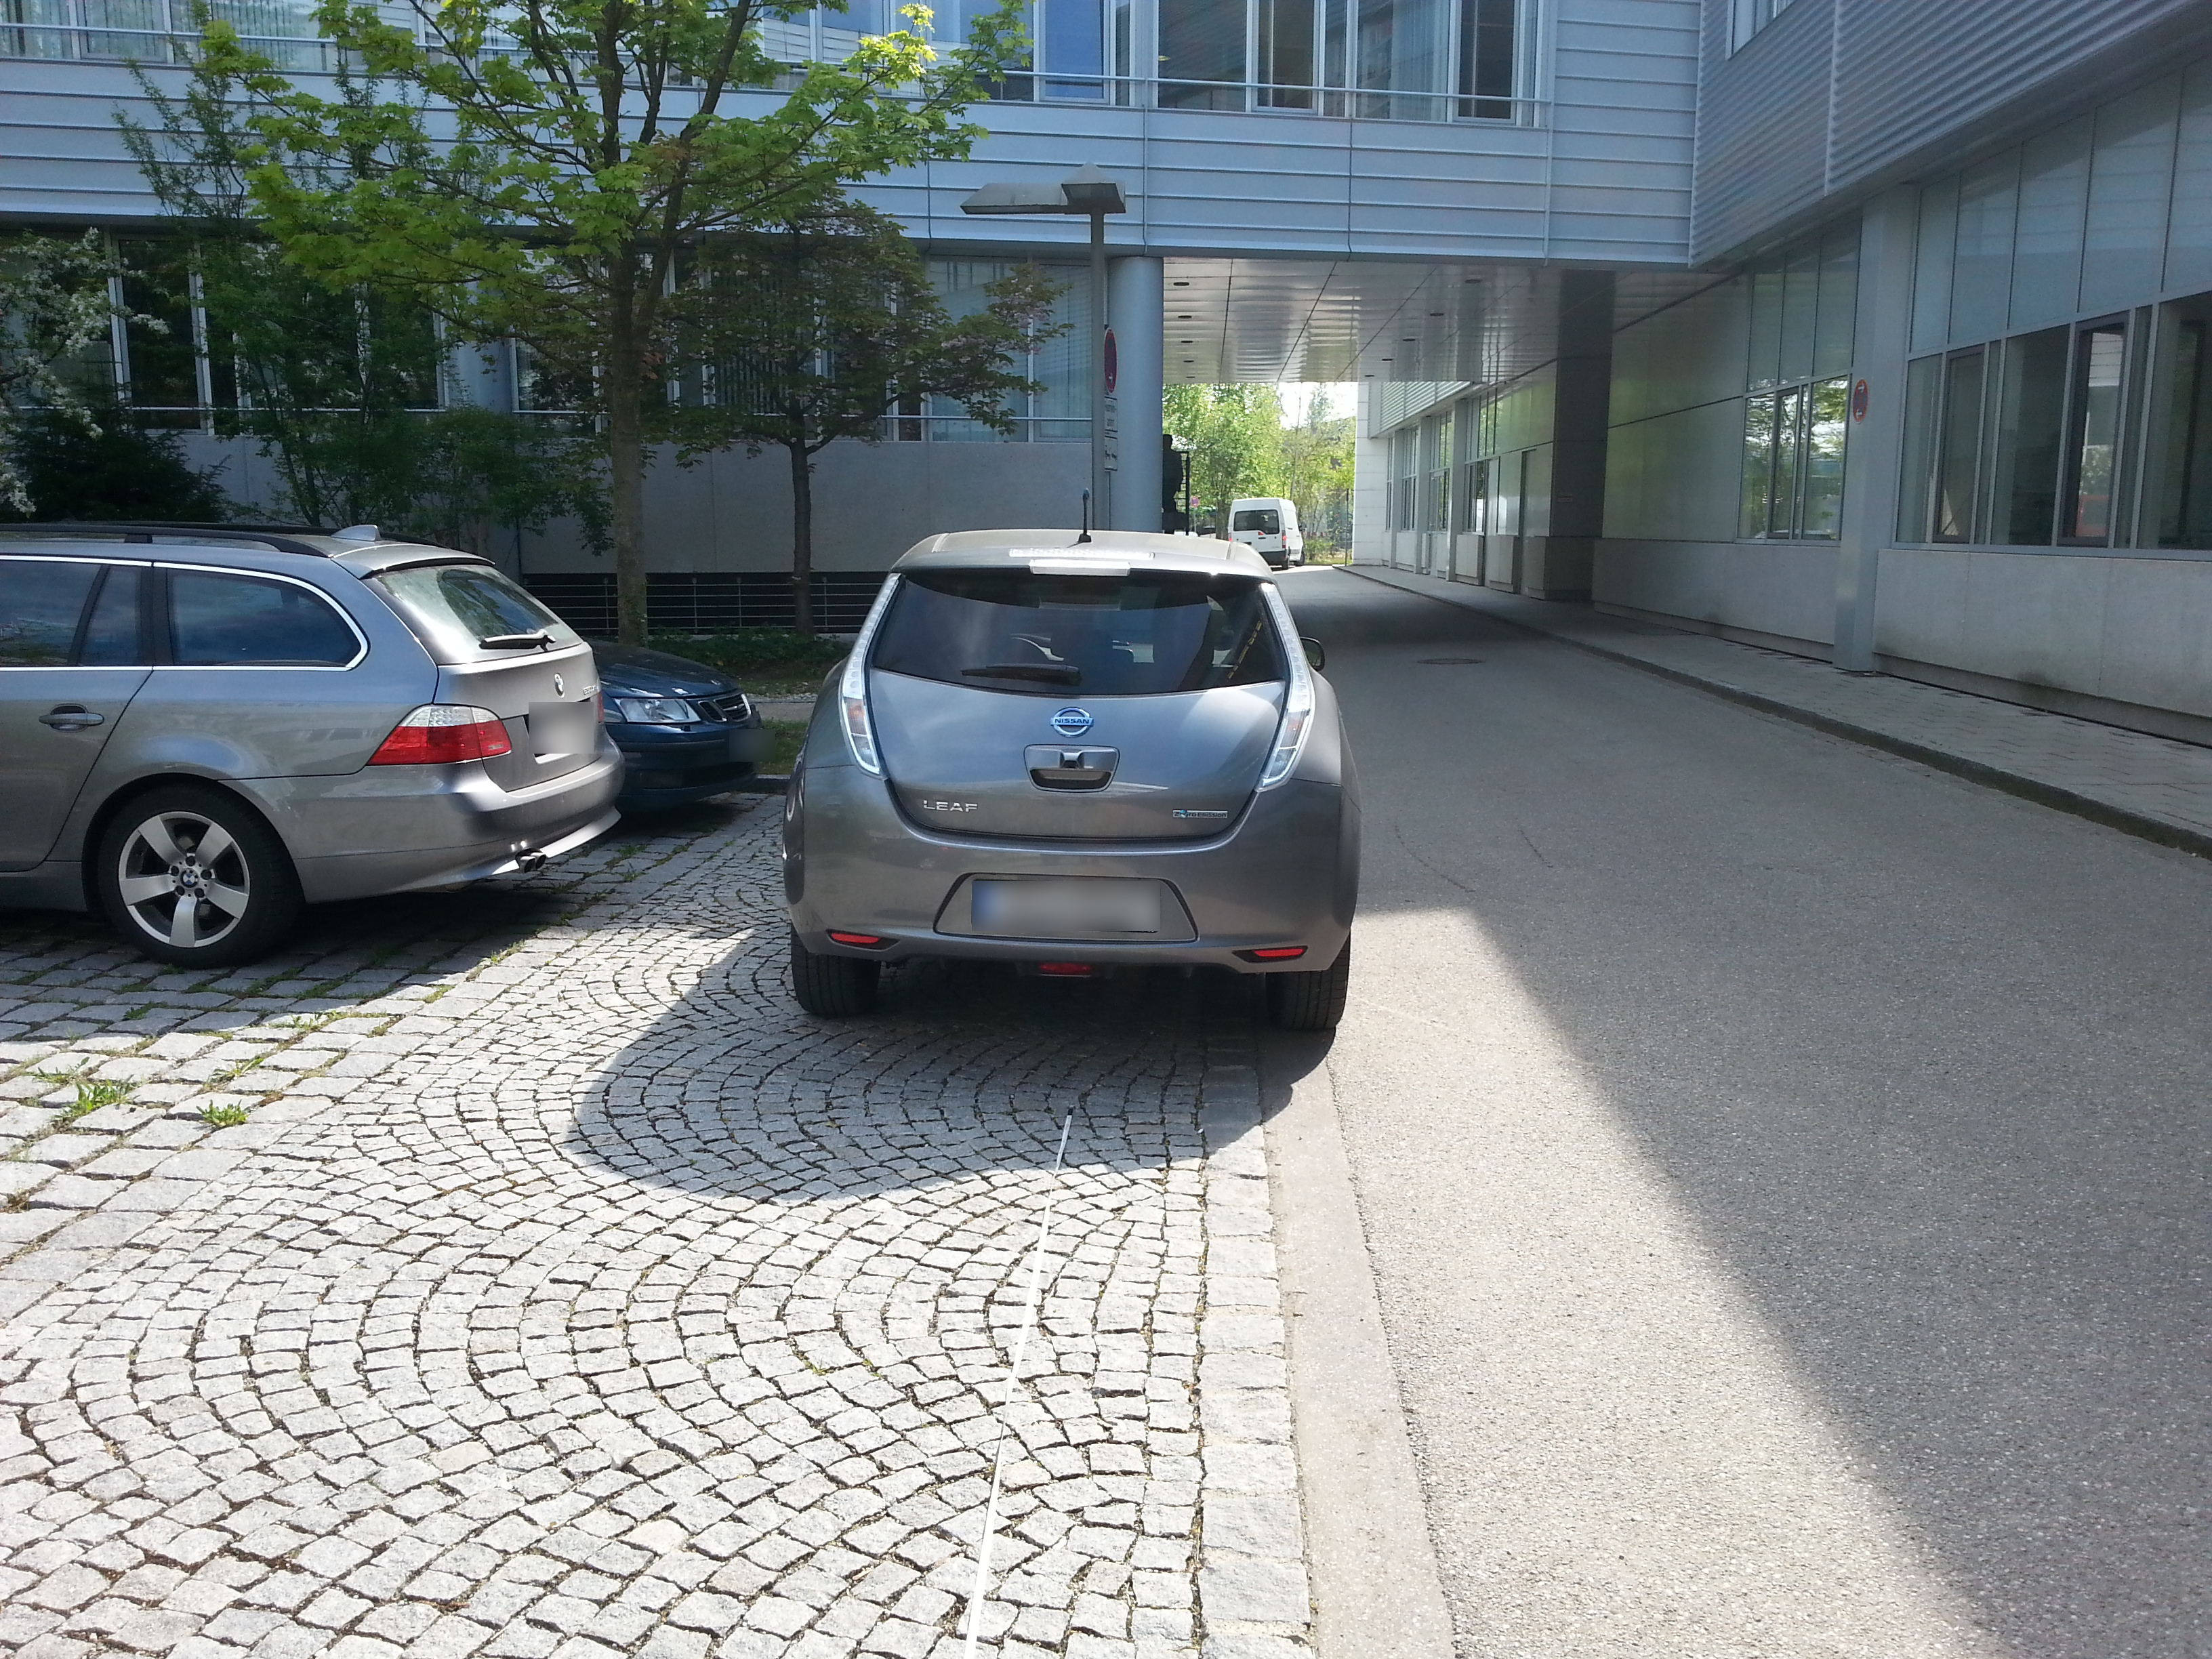
\includegraphics[width=0.75\linewidth]{img/elwoplate5m.jpg}
\caption{Distance of 5 meters to the vehicle}
\end{subfigure}
\begin{subfigure}[b]{0.5\textwidth}
\centering
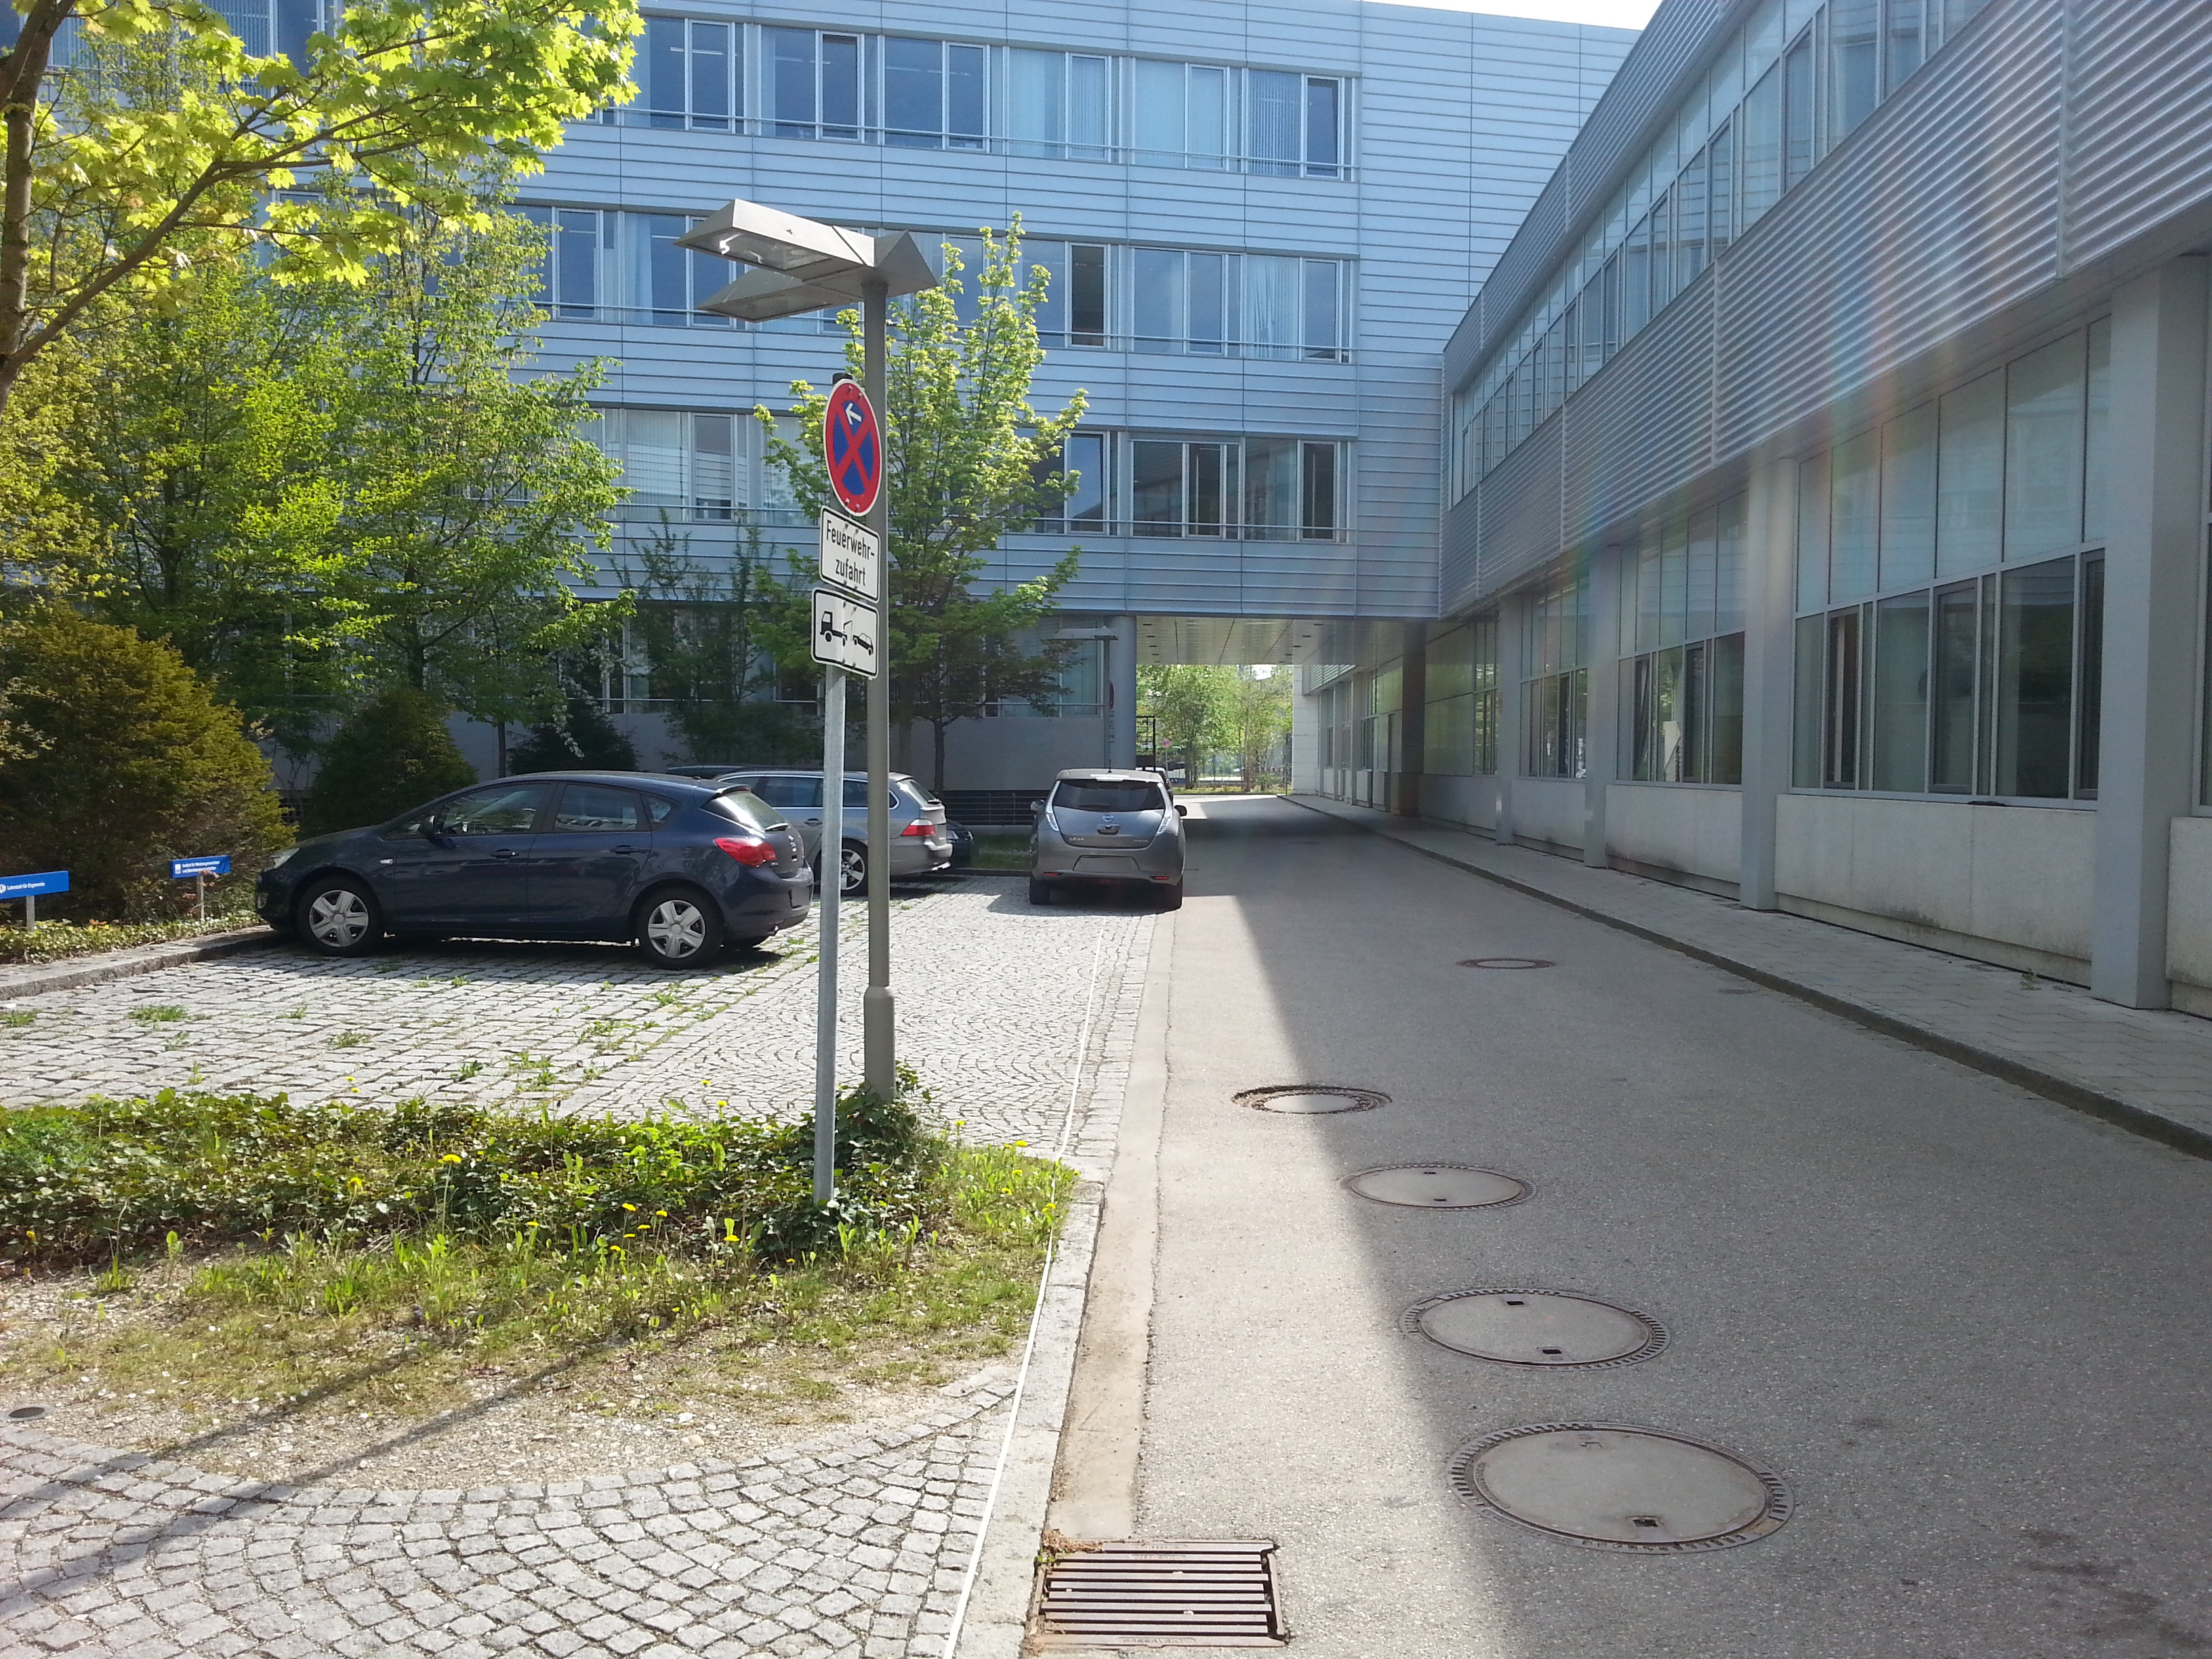
\includegraphics[width=0.75\linewidth]{img/elwoplate20m.jpg}
\caption{Distance of 20 meters to the vehicle}
\end{subfigure}
\begin{subfigure}[b]{0.5\textwidth}
\centering
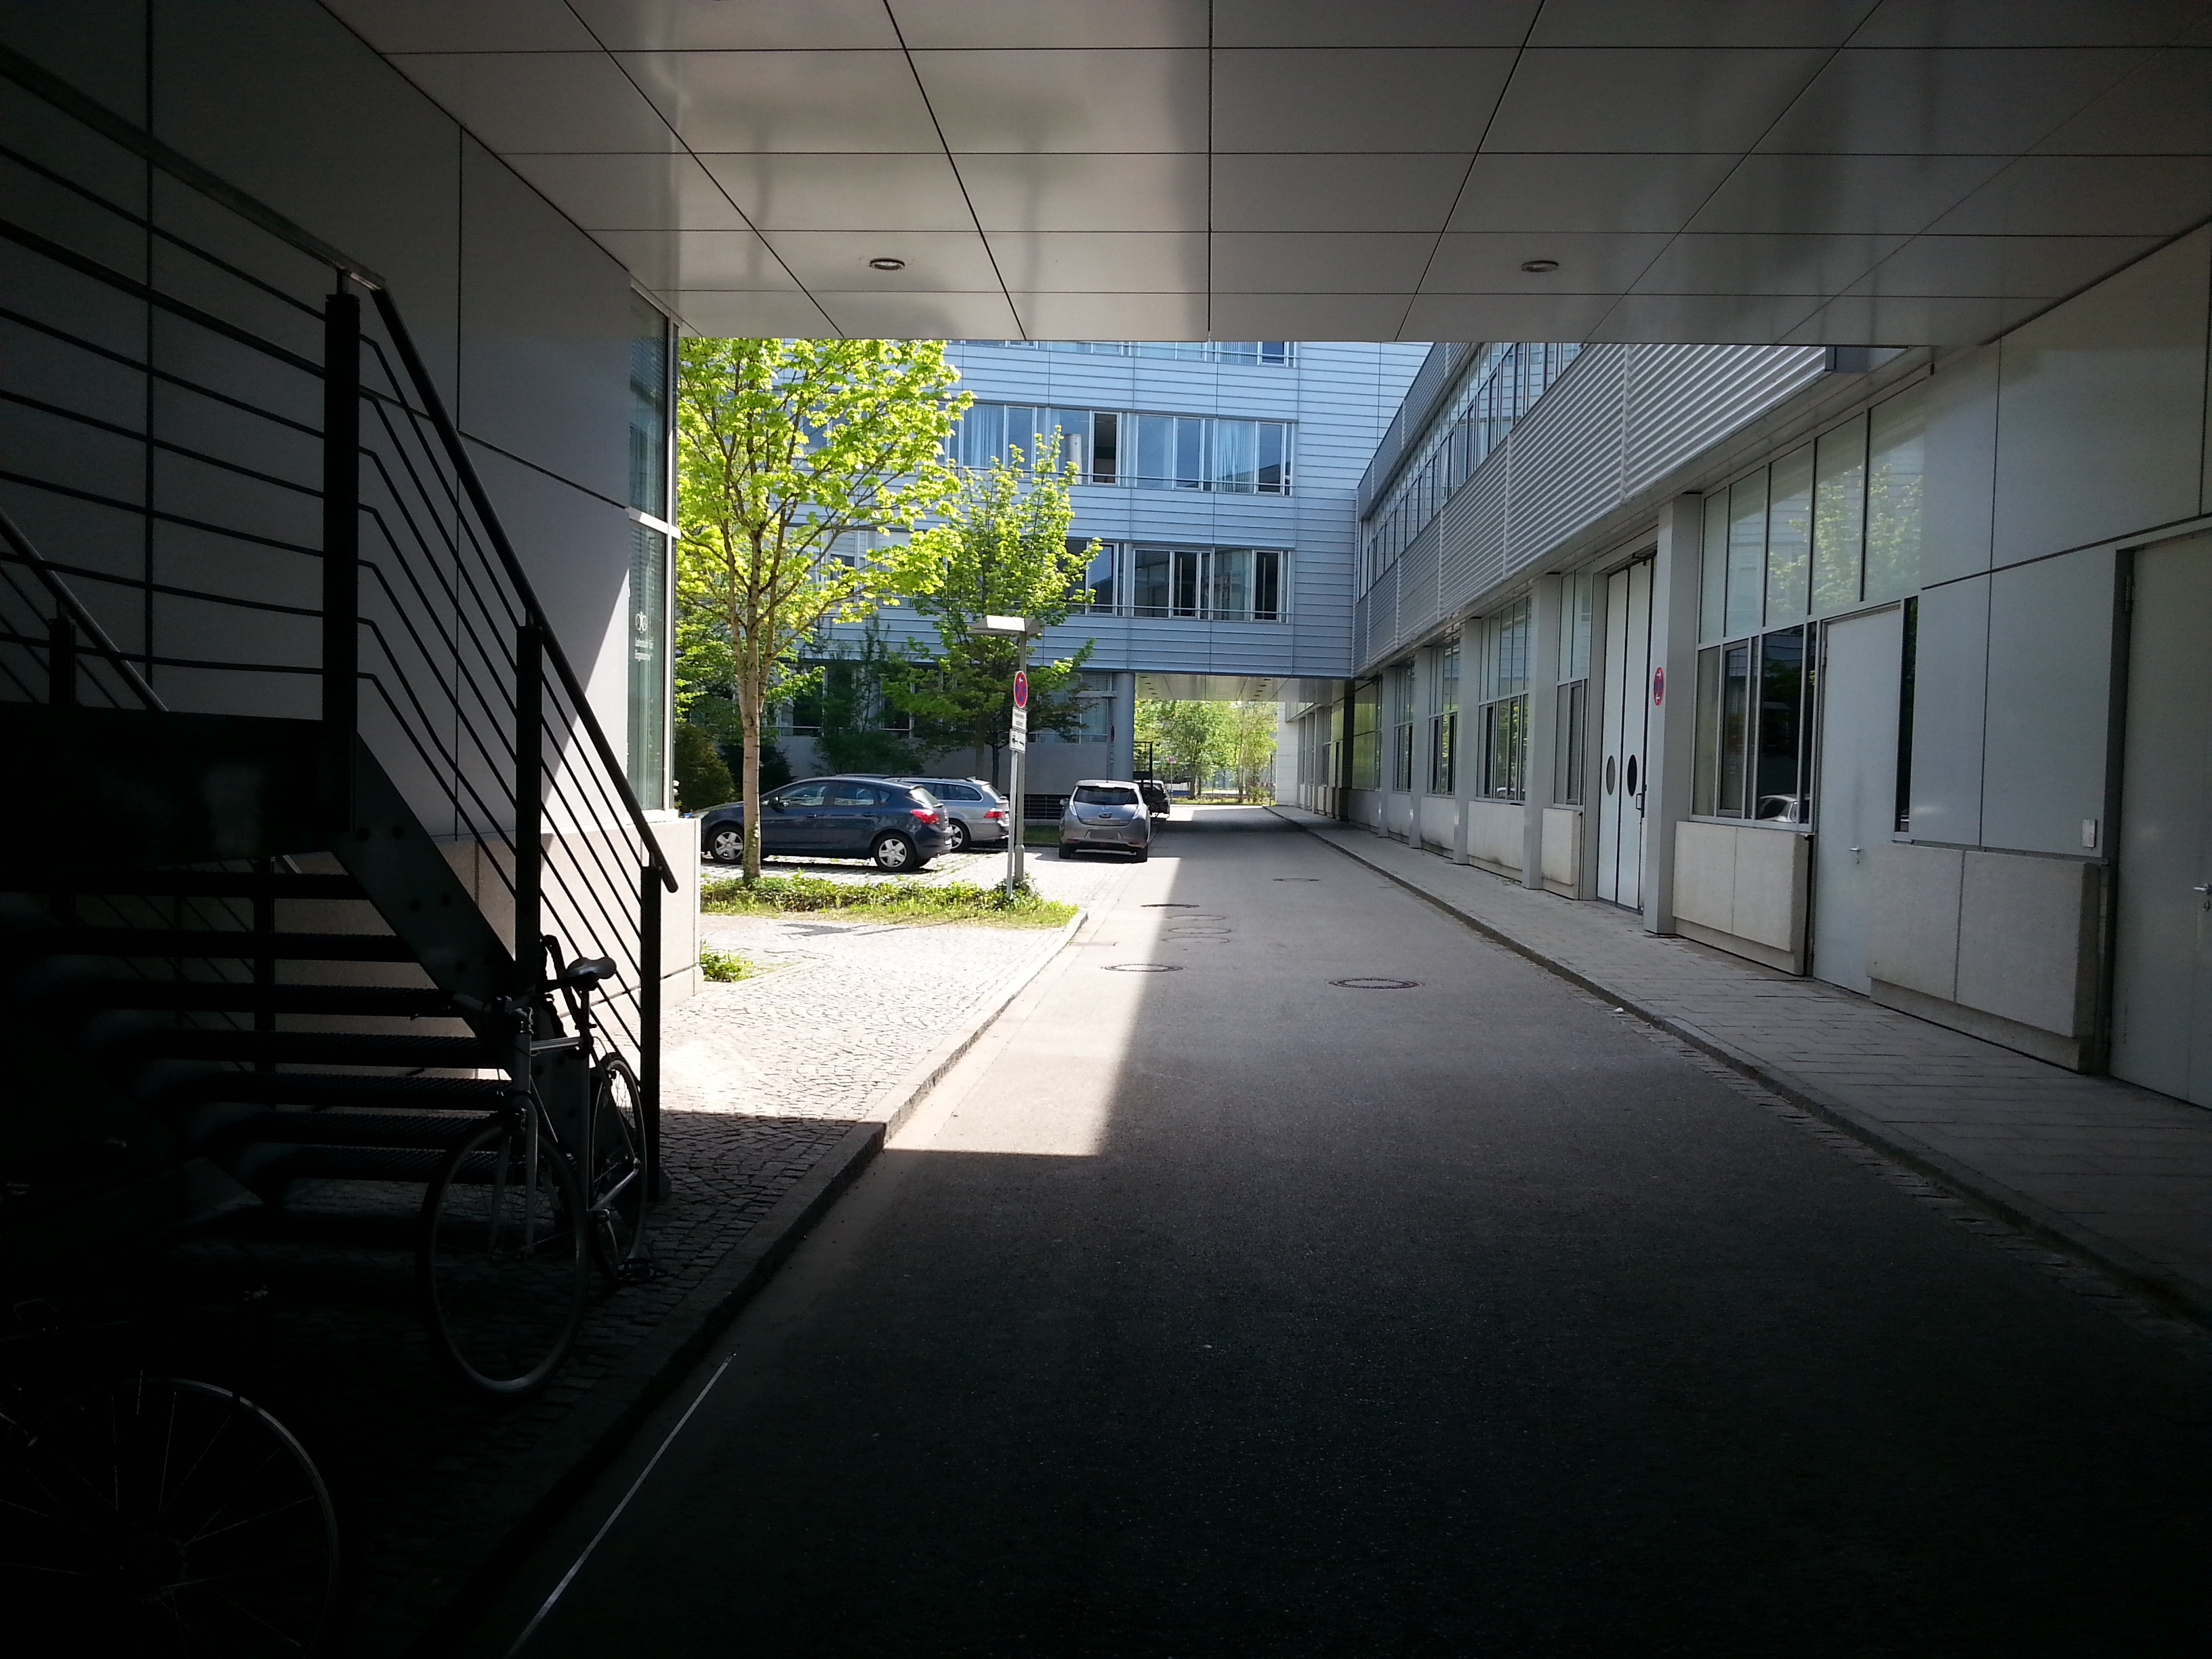
\includegraphics[width=0.75\linewidth]{img/elwoplate35m.jpg}
\caption{Distance of 35 meters to the vehicle}
\end{subfigure}
\begin{subfigure}[b]{0.5\textwidth}
\centering
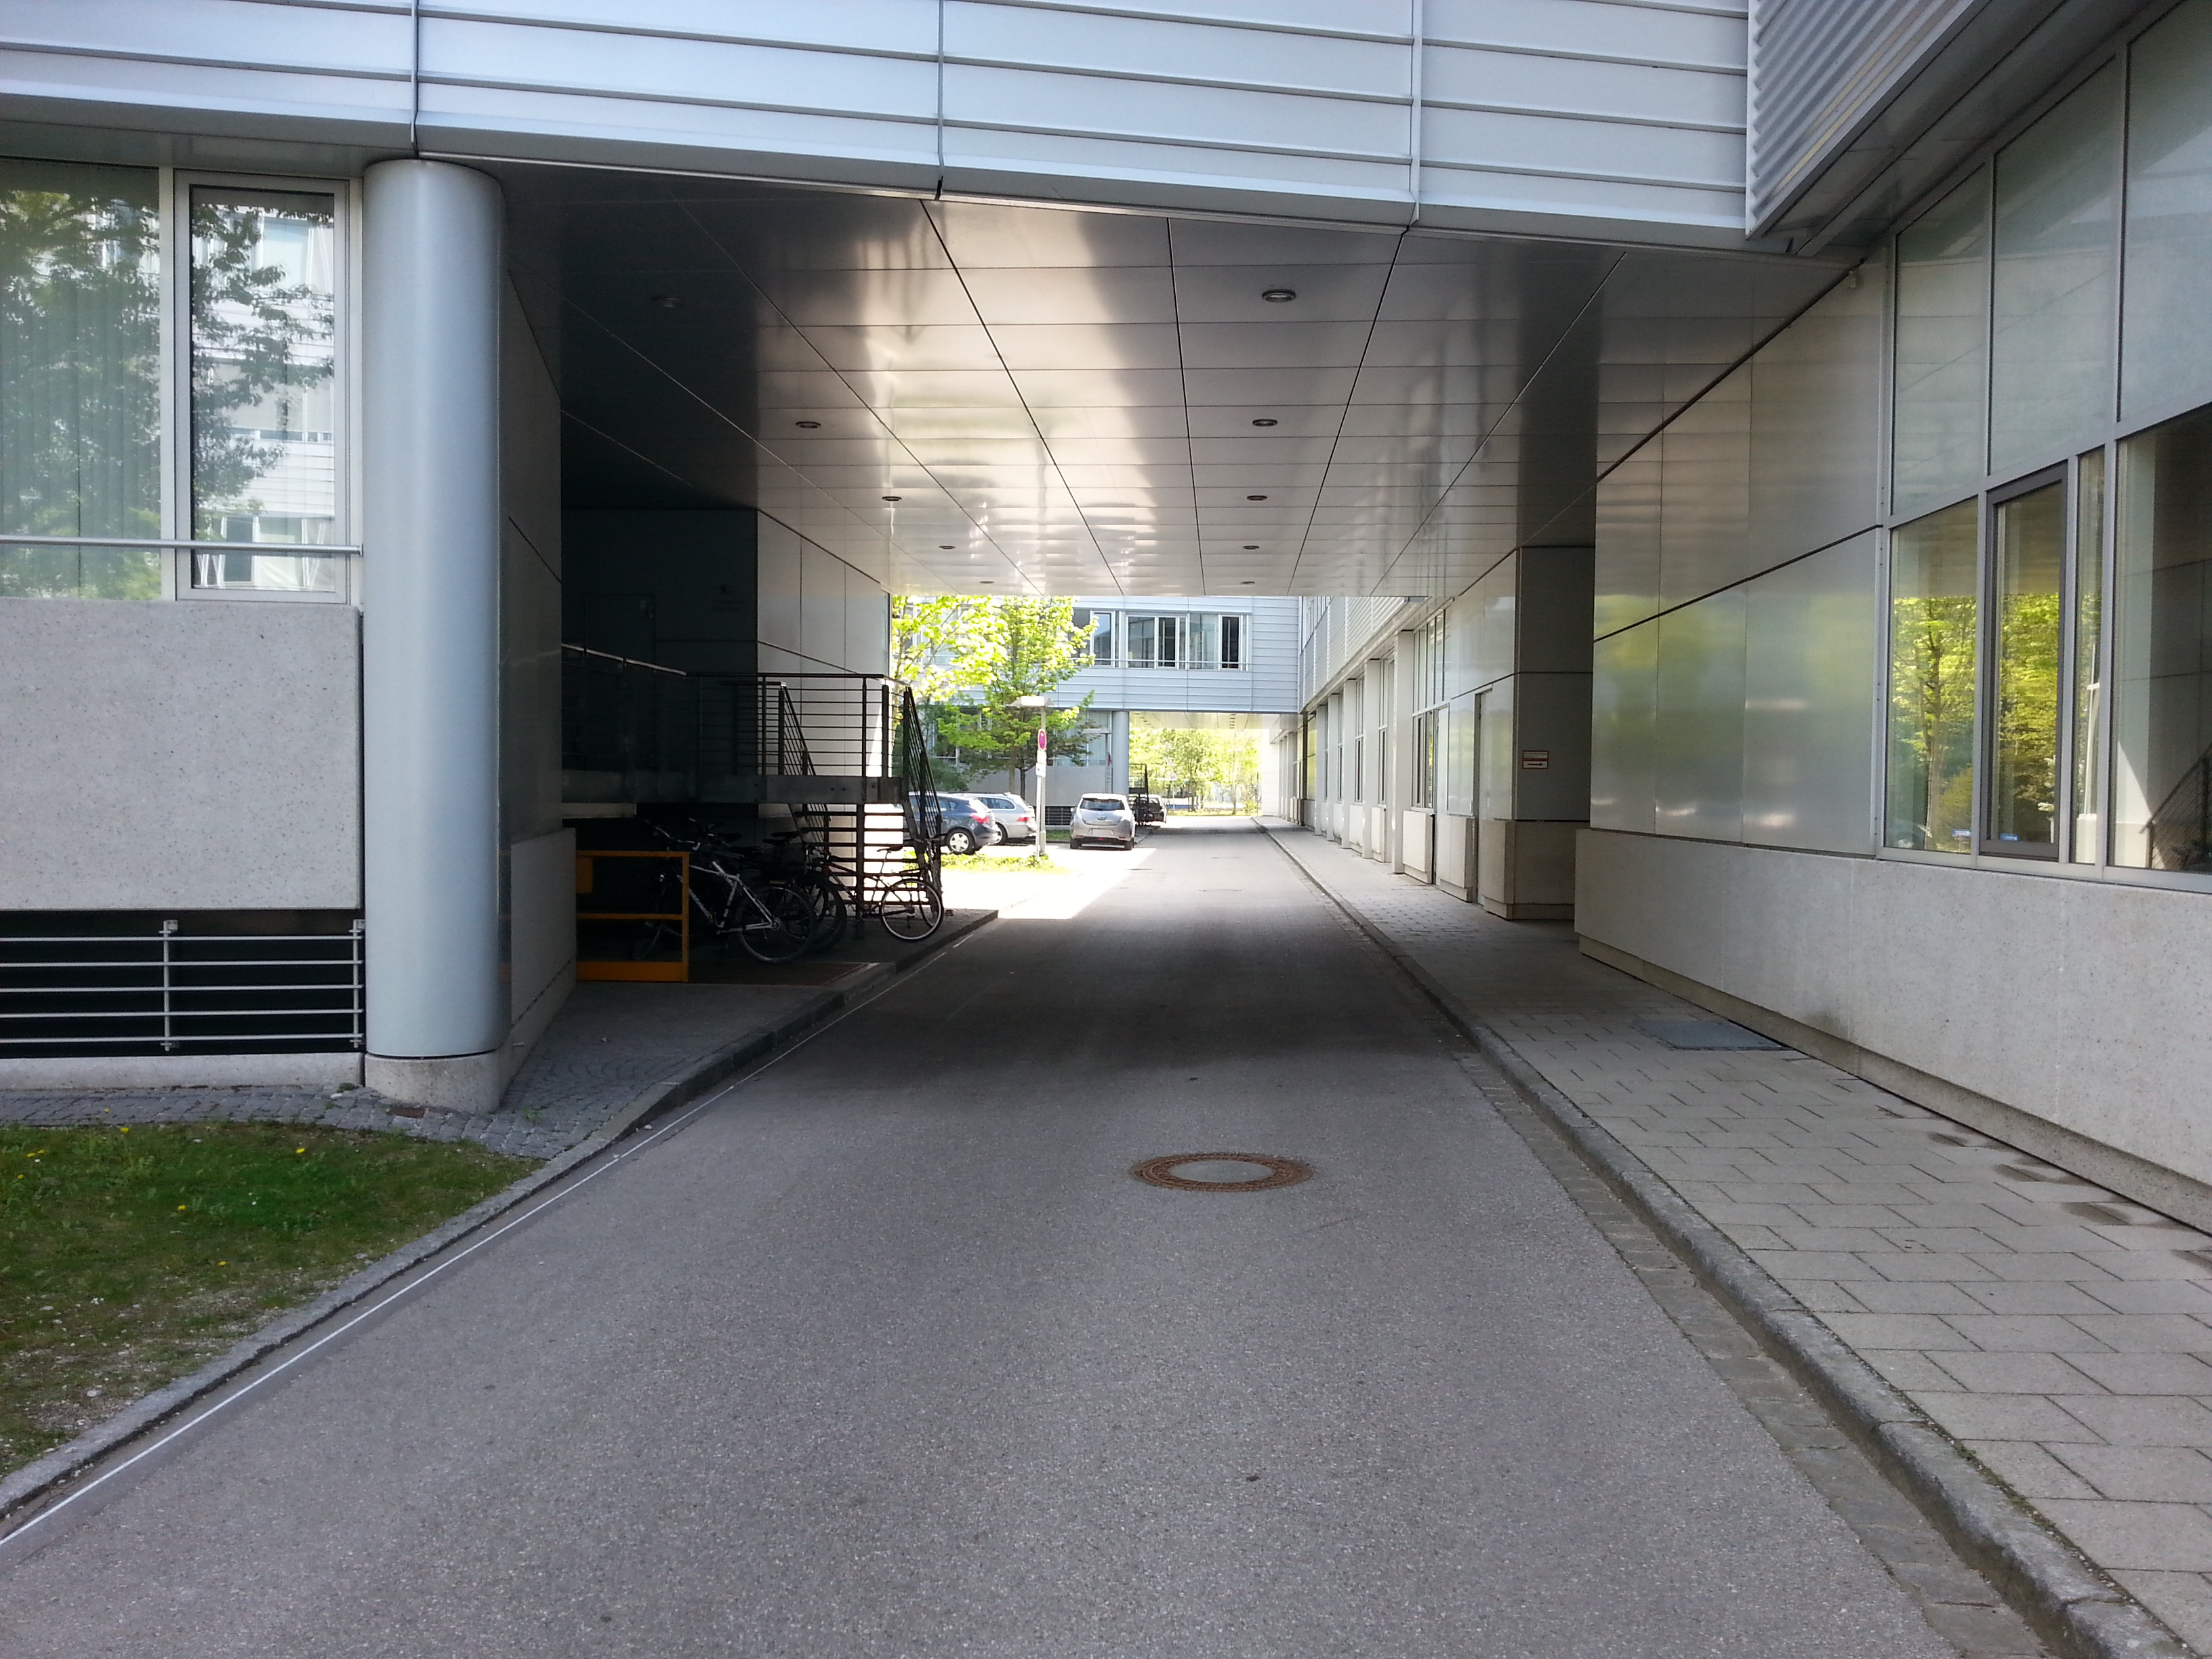
\includegraphics[width=0.75\linewidth]{img/elwoplate50m.jpg}
\caption{Distance of 50 meters to the vehicle}
\end{subfigure}
\caption{Sample of images at different distances from the testing vehicle}
\label{fig:distance-pictures}
\end{figure}

In the figure~\ref{fig:distance-curve-fitting} are displayed as red points, the
measurements obtained from each image. As you can see, this points follows an
exponential function. In order to be able to make a prediction of the distance,
it was decided to fit a exponential model to this data points. The exponential
model selected for this task is given by the next formula

\begin{equation}
    \mathcal{M}(x) = a \cdot \exp(b \cdot x) + c \cdot \exp(d \cdot x)
    \label{eq:distance-curve-model}
\end{equation}

\begin{figure}[h]
\centering
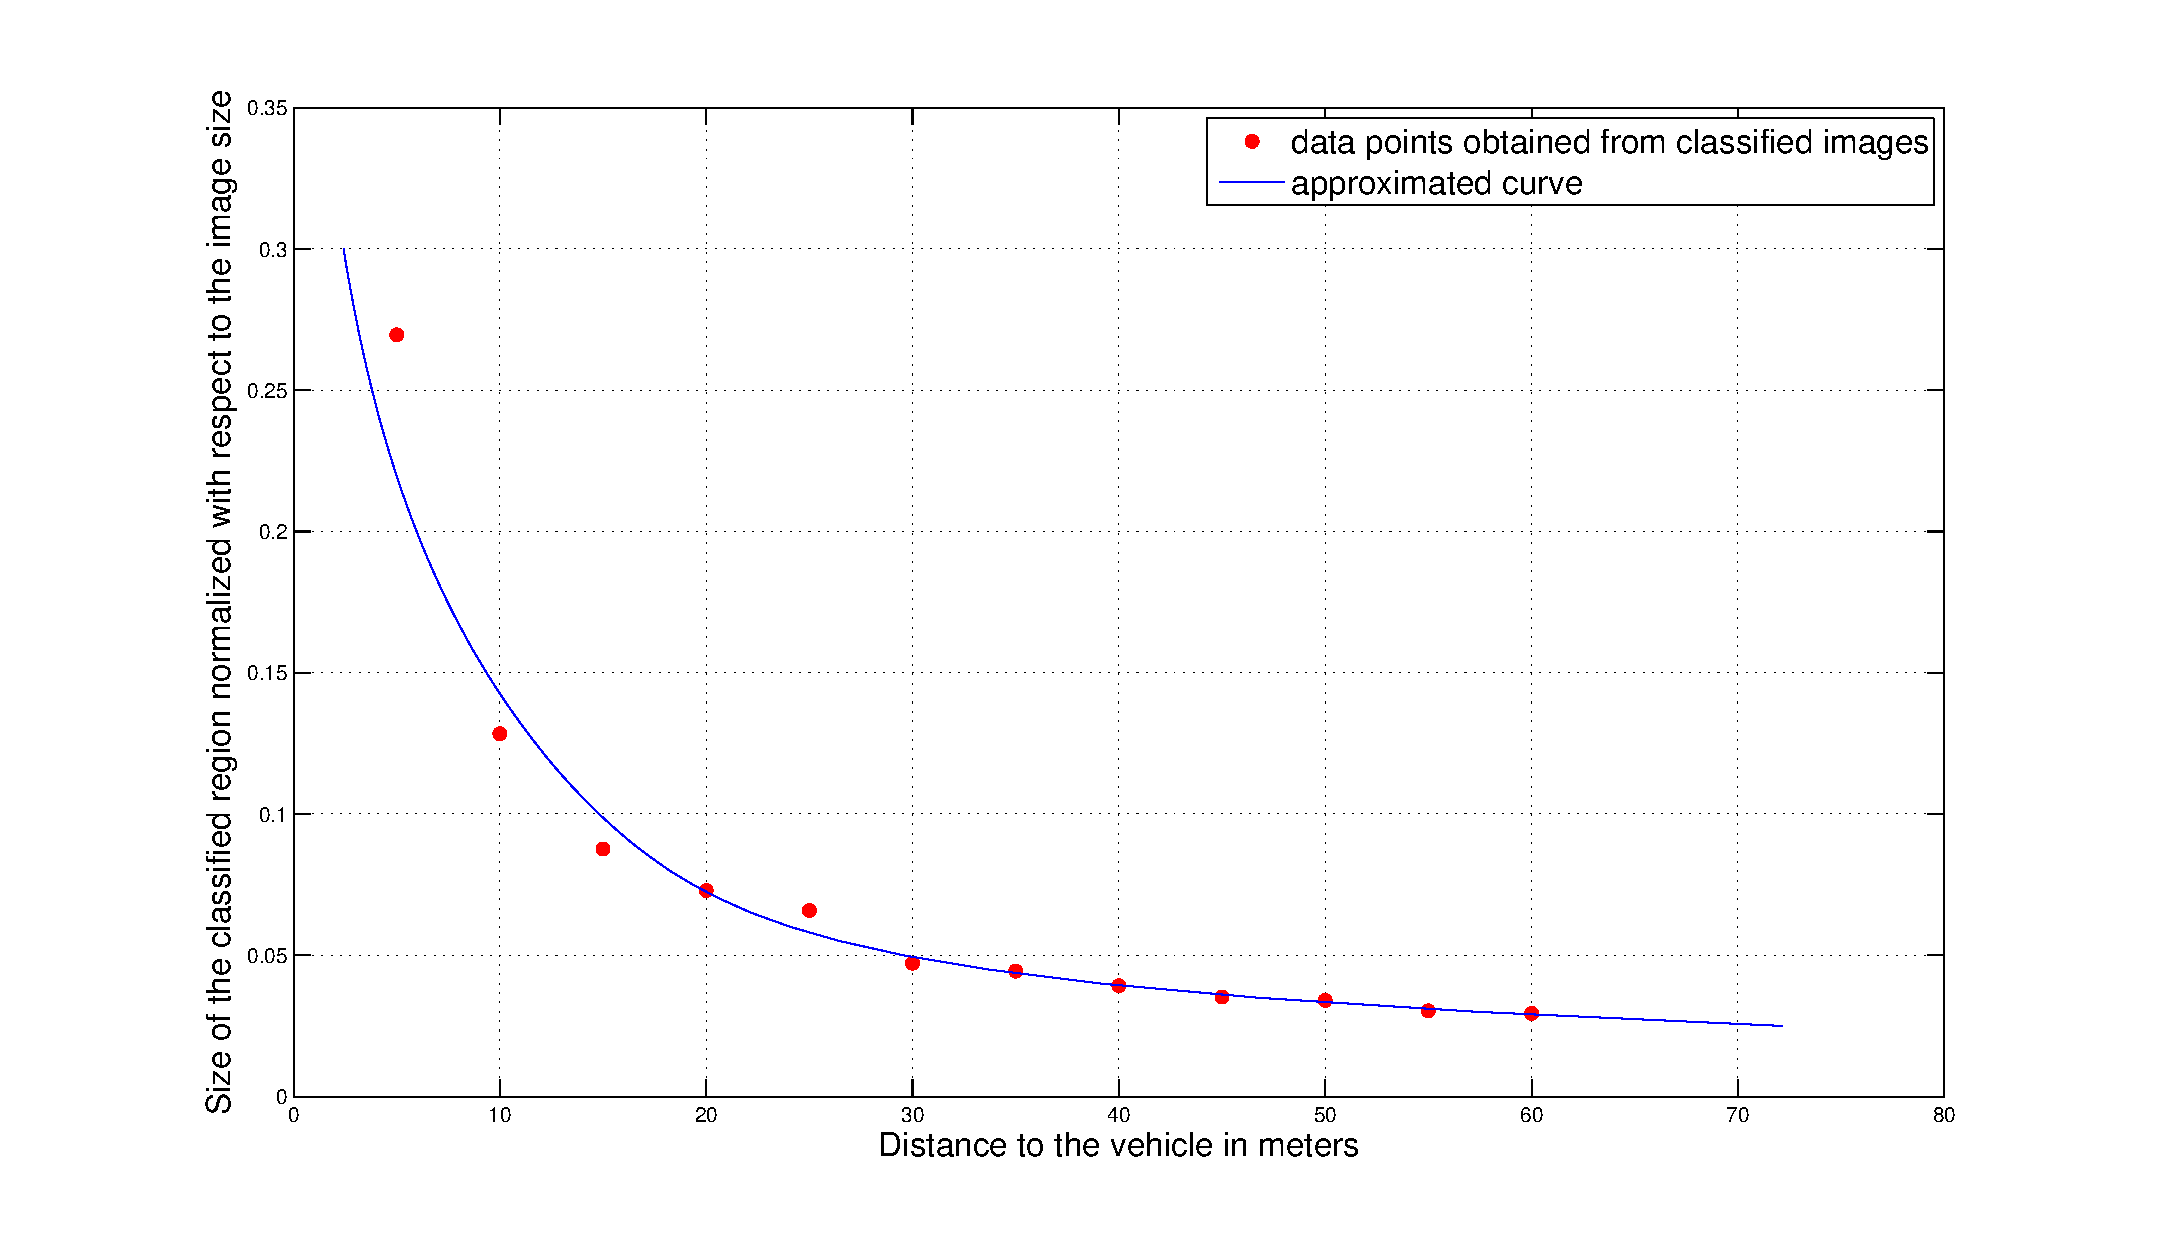
\includegraphics[width=\linewidth]{img/fitted_curve.eps}
\caption{Curve fitting for distance approximation from classification region
    size. In the horizontal axis is the distance to the vehicle in meters.
In the vertical axis is the normalized region size containing the vehicle. The red
points represent the measure obtained from each image. The blue curve is the predicting model fitted to the data points.}
\label{fig:distance-curve-fitting}
\end{figure} 

It is important to point out that this approximated model is directly related to
the classifier itself. This is because the measurements from the pictures are
obtained through it. This implies that whenever the classifier is changed, a new
coefficients are need to be calculated.

In order to do this relation invariant to the image resolution, we normalize the
size in pixels of the region containing the vehicle with the total width of the
image. With this results we can find  an approximated distance to the
vehicle, giving an initial solution to the problem of distance estimation.

% section Distance estimation (end)

\section{Vehicle tracking} % (fold)
\label{sec:vehicle-tracking}

Once the classification is done, the estimation of the distance should be
associated to its respective vehicle. For this reason, it is necessary to track
the vehicles appearing in the image. To do this, we observe that each vehicle has 
a certain motion and position from frame to frame. Ideally, given the
assumptions we made about the fixed camera view, the motion and position of each
vehicle should be similar between frames.

Traditionally, the \textit{optical flow} is known as the apparent motion of
objects in the image caused by the relative motion of the camera and the scene.
This concept was study in maybe one of the most influential works in computer 
vision done by \cite{lucas-kanade}. In this approach, the image derivatives are
used to obtain a motion vector inside a small windows partitioning the image. 
Later, these velocity vectors can be used with a mean-shift approach to get 
the final position of the object.

In principle, this technique could be used together with the classifier, giving
the last one a starting point for the tracking. This is commonly done because
usually the classification takes more time than the tracking. In this project we
tested this approach by switching between a \textit{detection phase} and a
\textit{tracking phase} periodically. This has proven to be more fast than
performing a detection on each frame.

Now we can assign an identification number to each vehicle by
thresholding the similarity between the classification regions. Basically, if a 
rectangle appearing in two consequent frames have similar position and size, these
two are consider to correspond to the same vehicle and an identification number
is assigned. 

In figure~\ref{fig:tracking} you can see four sequential images separated by 20
frames in between. The color of the bounding boxes correspond to the identification 
number assigned to a vehicle. For example, the vehicle inside the
yellow box is tracked successfully in the entire sequence. Nevertheless, when a
vehicle is not correctly classified in a particular frame, the tracking is lost.
You can see this in the same figure, the vehicle inside the pink bounding box is 
later labeled with the blue color, meaning that the tracking was lost at some point 
and then rediscovered by the classifier. 

\begin{figure}[t]
\centering
\begin{subfigure}[b]{0.4\textwidth}
\centering
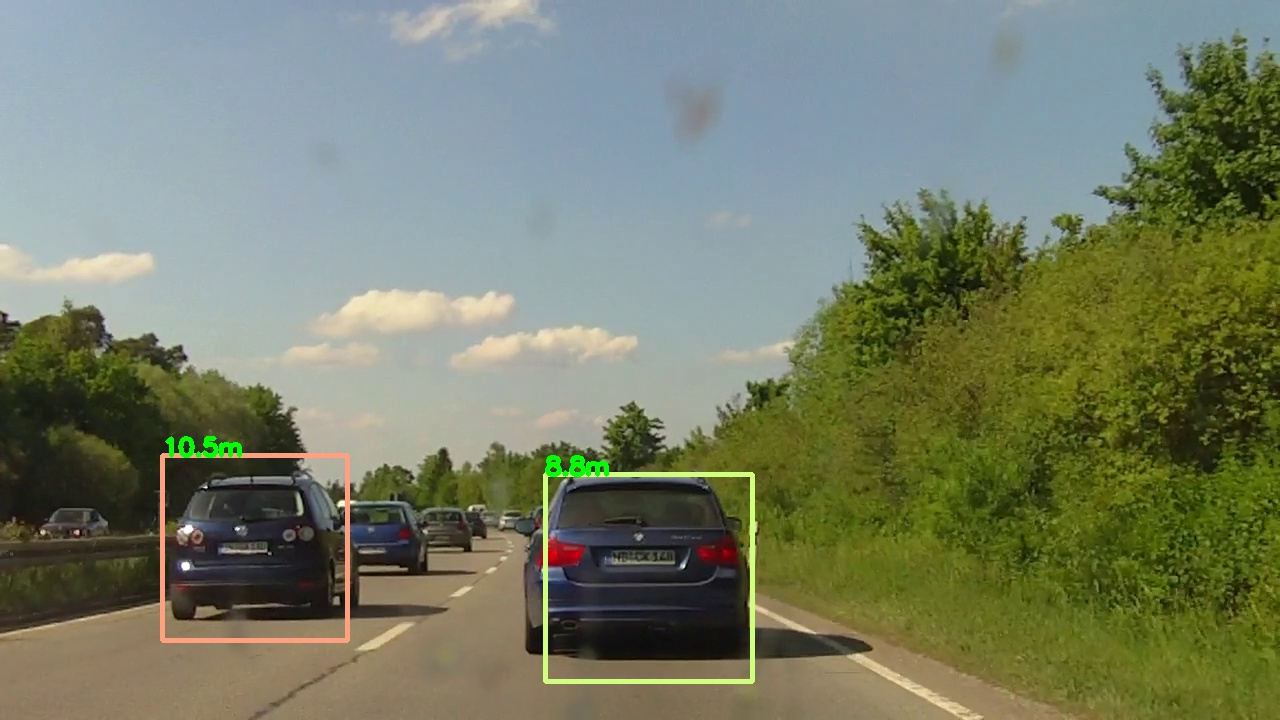
\includegraphics[width=0.9\linewidth]{img/tracking1.jpg}
\vspace{5mm}
\end{subfigure}
\begin{subfigure}[b]{0.4\textwidth}
\centering
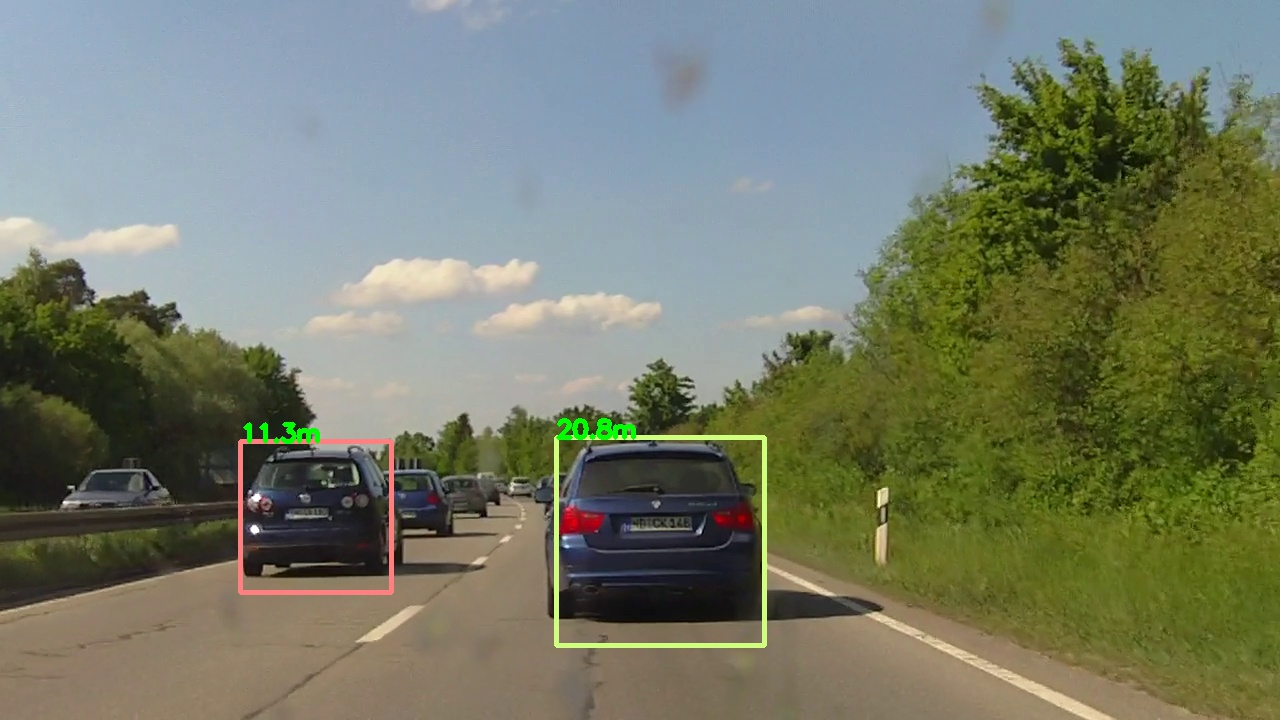
\includegraphics[width=0.9\linewidth]{img/tracking2.jpg}
\vspace{5mm}
\end{subfigure}
\begin{subfigure}[b]{0.4\textwidth}
\centering
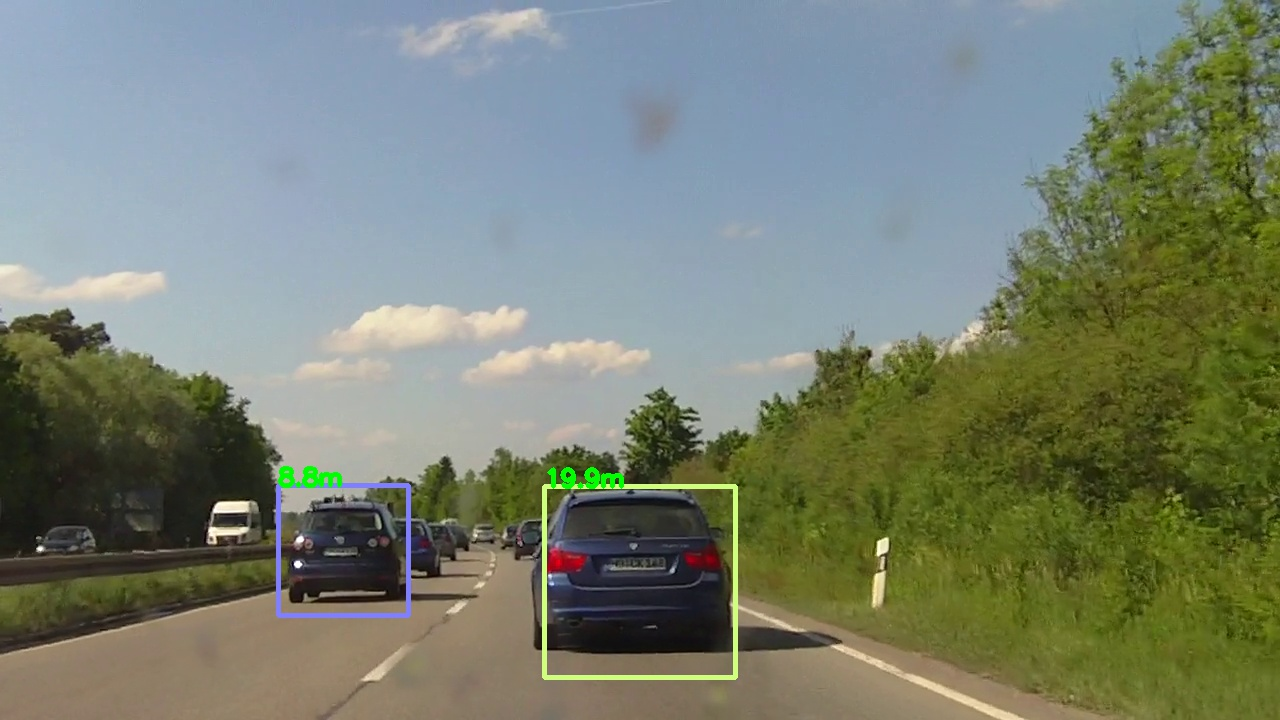
\includegraphics[width=0.9\linewidth]{img/tracking3.jpg}
\end{subfigure}
\begin{subfigure}[b]{0.4\textwidth}
\centering
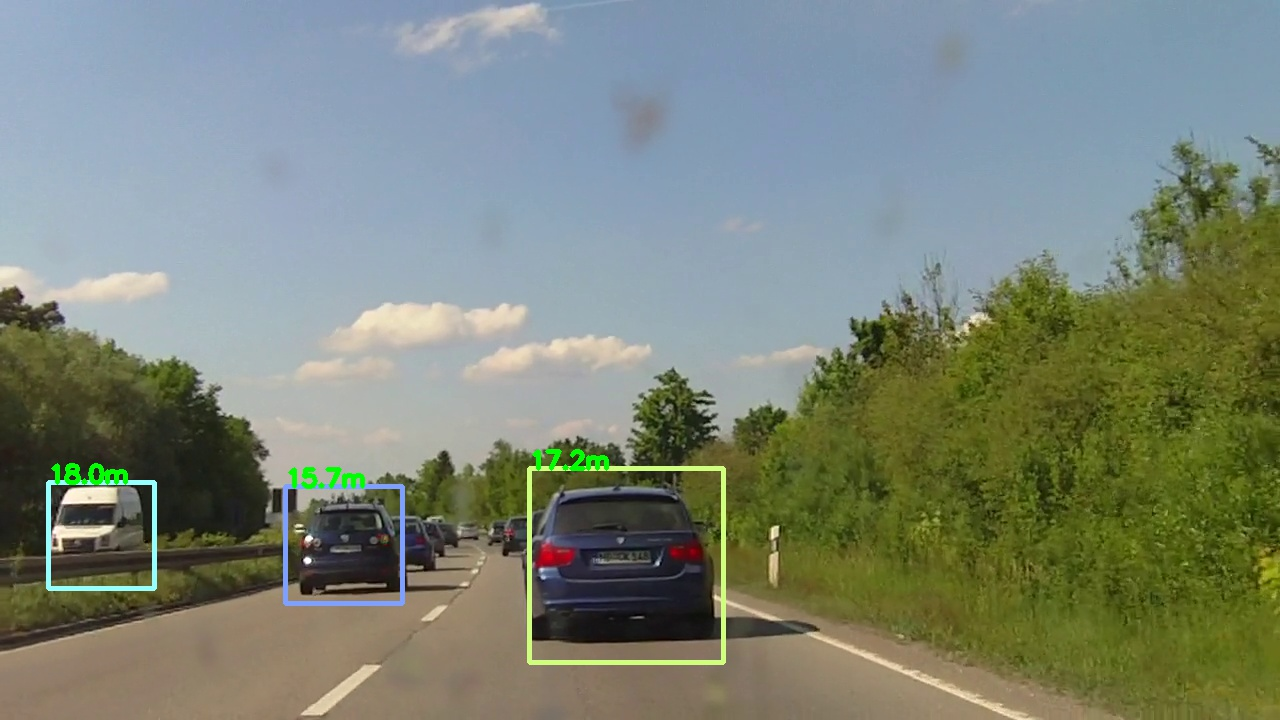
\includegraphics[width=0.9\linewidth]{img/tracking4.jpg}
\end{subfigure}
\caption{Tracking of vehicles. The pictures shown here have 20 frames of
separation.}
\label{fig:tracking}
\end{figure}

% section vehicle-tracking (end)

\section{Speed estimation} % (fold)
\label{sec:speed-estimation}

The missing peace to obtain the metric is to estimate the speed of vehicle with
the on-board camera. In principle for this purpose, the same concept of
\textit{optical flow} explained in the previous section could be applied.
Nevertheless, nowadays is normal that Smart-phones have \textit{Global
Positioning System} or GPS for short. With this technology is possible to
estimate the speed in a more easy and accurate way. This is done by first
estimating the position of the device.

The GPS can estimate the actual position of the device using the received signal
of at least 4 GPS satellites. The distance to each satellite is calculated with
the transit time of the signal and the speed of light. There are other ways to 
calculate position of the device, for example the same idea can also be applied 
to the signal of antennas or even wireless networks access points.

It is trivial to calculate the speed once we have at least two measured
positions on time. The strength of this approach lies on the amount of
measurements we can obtain in time and their accuracy.

% section speed-estimation (end)
